\section{Real navigation scenario} \label{sec:real-scenario}
Authentic data taken from previously recorded Nessie mission were used to simulate the algorithm ``offline'' as the part of the stage intended for testing and correcting. Besides, being able to repeat the same measurement scenario enables more insight in filtering process and benefits of fusing together the sensor data. \textit{.bag} files (\url{http://www.ros.org/wiki/}) containing recorded real-time messages with sensor measurements, were used as source. Furthermore, it allows designing the code in its original C++ form that will require little modification once deployed on the vehicle in form of ROS package since \textit{.bag} files emulate authentic messages and timestamps. One of the deficiencies of the evaluation of localisation results is the fact that there is no exact ground truth to compare the result with. Dead reckoning localisation substituted with occasional LBL position updates was compared with the localisation obtained after filtering (Figures ~\ref{fig:auv-sim-straight2}, ~\ref{fig:auv-sim-straight1}) for the recorded straight line trajectory mission. 

\T{Selecting a heading measurement with good performance}
For a high-end underwater vehicle such as Nessie, supplied with FOG-based INS, DVL and LBL, main source of navigation error is influenced by transformation of vehicle-referenced velocities to world-referenced velocities \cite{bahr08}, particularly due to yaw (heading) measurement errors. Yaw can be measured using several devices, each having different accuracy and performance. Simulation with data from previous missions was carried out to see which device gives the best performance for a given underwater vehicle. 

Heading calculated by integrating FOG's yaw rate - tends to be accurate and fast, less prone to noise. Nevertheless, it is calculated each time by appending yaw rate value integrated in time on the previous yaw value (relative measurement). Therefore, it is sensible on initial absolute heading measurement. In case initial yaw is imprecise, a constant bias exists in yaw measurement (Figure ~\ref{fig:auv-sim-straight1}). Constant bias causes sudden steps in position estimate obtained using EKF. This is expected scenario since the sensor responsible for measuring initial heading is magnetic compass, device sensitive to disturbances coming from environment (Figure ~\ref{fig:magnetic-disturb}). In real experiments biggest obstacle was proper calibration of magnetic compass. In practice, tests have showed many failures in compass heading measurement, possibly due to calibration and magnetic declination. There is yet space to do more testing with better compass tuning. To overcome the problem of accurate yaw measurement, EKF used in experiments will either ignore the yaw measurement (it is possible since sensor fusion successfully compensates missing heading information with yaw rate obtained from FOG) or use it with high variance assigned to yaw measurement. 
%Finally, initial heading is given with magnetic compass.

\T{Loch Earn dataset - straight line movement}: Example of basic EKF localisation using inertial measurements aided with LBL acoustic positioning system was tested on straight line movement of approximately 80 m length, recorded at the lake Loch Earn. For simulation purposes, sensor measurements are stored in a \textit{.bag} file, that can be replayed, producing real-time messages of sensor measurements as they originally occurred. At this point, it is important to revise which sensors were used, their main features and, finally, filtering parameters. 

Standard sensor configuration comprising of pressure sensor, magnetic compass, FOG and DVL is used in the mission. Absolute position correction was carried out using LBL system. Important fact is that the heading was measured with magnetic compass only at the beginning. Later on, it kept being calculated by integrating yaw rate obtained from FOG. Alternative solution for the heading measurement would be the usage of compass for direct acquiring of yaw, but such option exposed calibration difficulties. Result of EKF localisation algorithm was shown in north-east map (Figure ~\ref{fig:sim-straight2}, ~\ref{fig:sim-straight1}). Different parameter values for EKF were tested. Table ~\ref{tab:ekf-params} revises all filter parameters used for filter tuning, together with their role. Essentially, setting high standard deviation for a Gaussian of a certain parameter can be interpreted as having more uncertainty in value that it represents - whether it is a measurement uncertainty or uncertainty of the predicted value (model uncertainty). Therefore, we can choose to be confident in certain sensor measurement and/or certain model prediction, and observe the simulation outcome of such setting. Setting the parameters properly improves the performance of the filter.  
\addtocounter{footnote}{1}
\footnotetext[\value{footnote}]{as it appears in algorithm equations}  
\begin{table*}
\centering
	\caption{EKF navigation parameters.}
	\label{tab:ekf-params}
\begin{tabular}{llll}
\toprule
Parameter      &     Signature $^{\decimal{footnote}}$     &     Units     &    Description  \\
\midrule
                         & \multicolumn{3}{c}{standard deviation of the ... } \\ 
\multirow{1}{*}{SDNorth} & \multirow{1}{*}{$\sigma_{n}$} & \multirow{1}{*}{$m$} & \multirow{1}{*}{north observation} \\
\multirow{1}{*}{SDEast}  & \multirow{1}{*}{$\sigma_{e}$} & \multirow{1}{*}{$m$} & \multirow{1}{*}{east observation} \\
\multirow{1}{*}{SDDepth} & \multirow{1}{*}{$\sigma_{d}$} & \multirow{1}{*}{$m$} & \multirow{1}{*}{depth observation} \\
\multirow{1}{*}{SDAltitude} & \multirow{1}{*}{$\sigma_{a}$} & \multirow{1}{*}{$m$} & \multirow{1}{*}{altitude observation} \\
\multirow{1}{*}{SDu} & \multirow{1}{*}{$\sigma_{u}$} & \multirow{1}{*}{$\frac{m}{s}$} & \multirow{1}{*}{surge velocity observation} \\
\multirow{1}{*}{SDv} & \multirow{1}{*}{$\sigma_{v}$} & \multirow{1}{*}{$\frac{m}{s}$} & \multirow{1}{*}{sway velocity observation} \\
\multirow{1}{*}{SDw} & \multirow{1}{*}{$\sigma_{w}$} & \multirow{1}{*}{$\frac{m}{s}$} & \multirow{1}{*}{heave velocity observation} \\
\multirow{1}{*}{SDyaw} & \multirow{1}{*}{$\sigma_{\psi}$} & \multirow{1}{*}{$rad$} & \multirow{1}{*}{heading observation} \\
\multirow{1}{*}{SDpitch} & \multirow{1}{*}{$\sigma_{\varphi}$} & \multirow{1}{*}{$rad$} & \multirow{1}{*}{pitch observation} \\
\multirow{1}{*}{SDyawRate} & \multirow{1}{*}{$\sigma_{\dot{\psi}}$} & \multirow{1}{*}{$\frac{rad}{s}$} & \multirow{1}{*}{heading rate observation} \\
\multirow{1}{*}{SDpitchRate} & \multirow{1}{*}{$\sigma_{\dot{\varphi}}$} & \multirow{1}{*}{$\frac{rad}{s}$} & \multirow{1}{*}{pitch rate observation} \\
\midrule
                         & \multicolumn{3}{c}{standard deviation of the ... process noise} \\
\multirow{1}{*}{SDuModel} & \multirow{1}{*}{$\sigma_{\dot{u}}$}  & \multirow{1}{*}{$\frac{m}{s^{2}}$} & \multirow{1}{*}{surge acceleration} \\
\multirow{1}{*}{SDvModel} & \multirow{1}{*}{$\sigma_{\dot{v}}$}  & \multirow{1}{*}{$\frac{m}{s^{2}}$} & \multirow{1}{*}{sway acceleration} \\
\multirow{1}{*}{SDwModel} & \multirow{1}{*}{$\sigma_{\dot{w}}$}  & \multirow{1}{*}{$\frac{m}{s^{2}}$} & \multirow{1}{*}{heave acceleration} \\
\multirow{1}{*}{SDyawRateModel} & \multirow{1}{*}{$\sigma_{\dot{v}}$}  & \multirow{1}{*}{$\frac{rad}{s^{2}}$} & \multirow{1}{*}{yaw acceleration} \\
\multirow{1}{*}{SDpitchRateModel} & \multirow{1}{*}{$\sigma_{\dot{w}}$}  & \multirow{1}{*}{$\frac{rad}{s^{2}}$} & \multirow{1}{*}{pitch acceleration} \\
\bottomrule
\end{tabular} 
\end{table*}
Straight line movement with authentic sensor measurements recorded in Loch Earn was a basis for initial tests of the EKF localisation algorithm. Red line shows the dead reckoning navigation, which is directly updated with absolute position update (LBL). Dead reckoning uses values periodically ($\approx$5$Hz$) obtained from DVL and FOG (linear velocities: $u$ and $v$ and heading $\psi$, respectfully), and substitutes them into equations similar to ones used for north and east prediction within prediction model: 
$$ north = north + (uT+\dot{u}\frac{T^{2}}{2})\cos(\psi) - (vT+\dot{v}\frac{T^{2}}{2})\sin(\psi) $$
$$ east  = east  + (uT+\dot{u}\frac{T^{2}}{2})\sin(\psi) + (vT+\dot{v}\frac{T^{2}}{2})\cos(\psi) $$
% SDnorth/east = 5 $cm$, 
% SDnorth/east = 5 $cm$, 
\begin{figure}%[htb]
  \centering
    \subfigure[N/E localisation. Yaw was calculated by integrating yaw rate periodically measured using FOG.] {\label{fig:sim-straight2}
	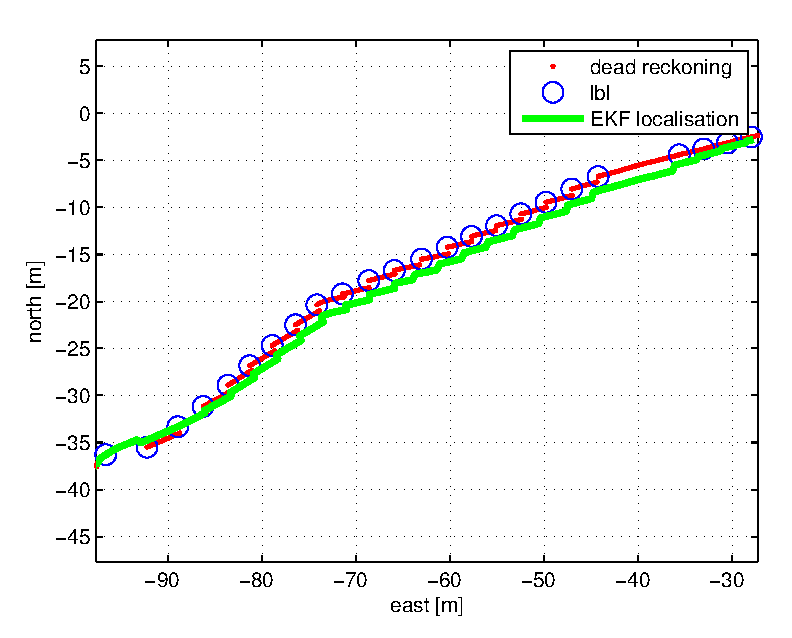
\includegraphics[width=0.48\linewidth]{simulations/fig/sim-straight2.eps}}
    \subfigure[Heading estimation. Biased yaw measurement not being corrected due to high confidence in yaw measurement.] {\label{fig:yaw-straight2}
    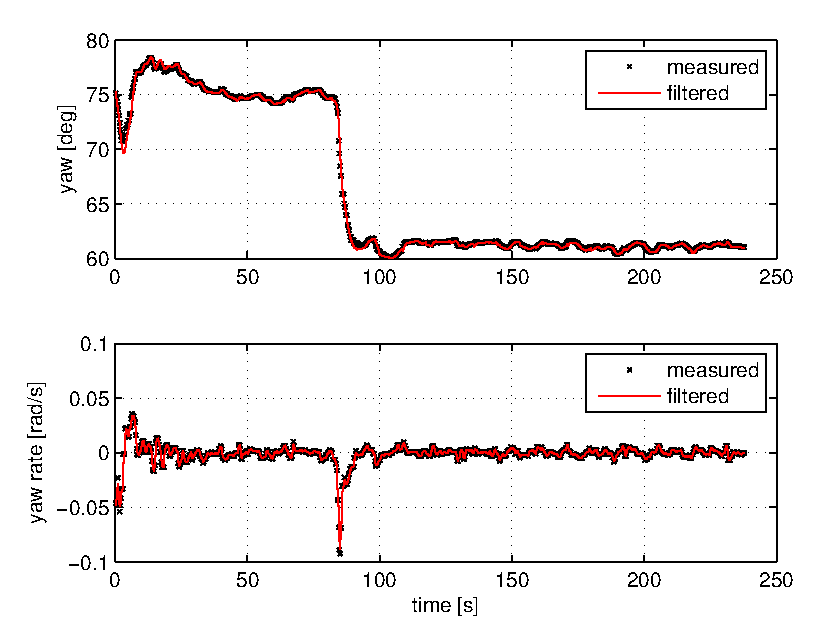
\includegraphics[width=0.48\linewidth]{simulations/fig/yaw-straight2.eps}} \\   
\caption{AUV localisation using EKF with high confidence in yaw measurement, SDyaw = 0.01$rad \approx 0.6 ^{\circ}$. SDyawRate = 0.004 $\frac{rad}{s}$, SDu/v = $1\frac{cm}{s}$.}

\label{fig:auv-sim-straight2}
\end{figure}
\begin{figure}%[htb]
  \centering
    \subfigure[N/E localisation. Yaw was calculated by integrating yaw rate periodically measured using FOG.] {\label{fig:sim-straight1}
	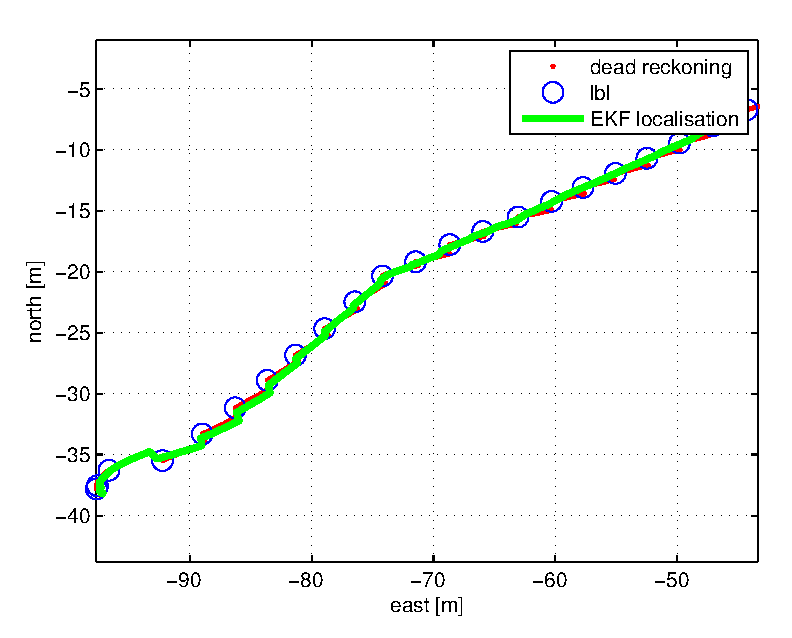
\includegraphics[width=0.48\linewidth]{simulations/fig/sim-straight1.eps}}
    \subfigure[Heading estimation. Biased yaw measurement is being corrected.] {\label{fig:yaw-straight1}
    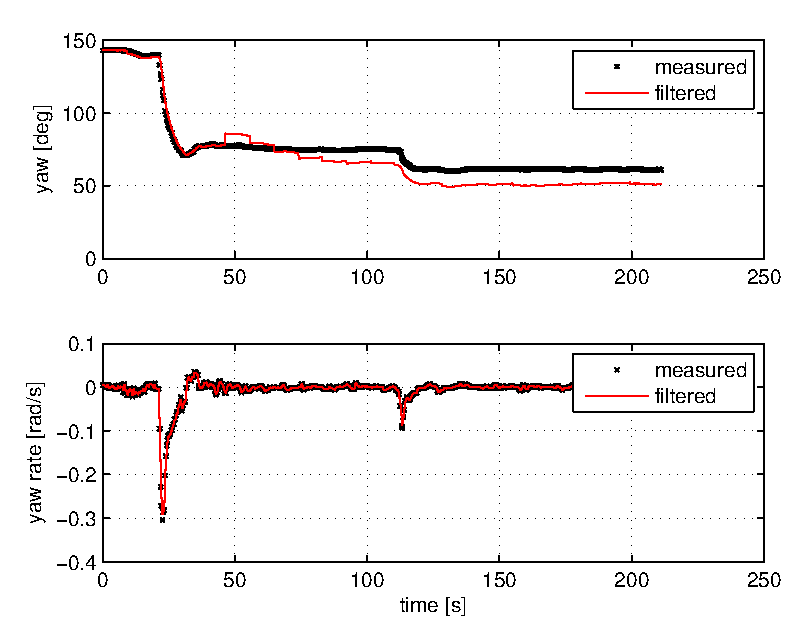
\includegraphics[width=0.48\linewidth]{simulations/fig/yaw-straight1.eps}} \\
\caption{AUV localisation using EKF with low confidence in yaw measurement, SDyaw = 0.2$rad \approx 11.5 ^{\circ}$. SDyawRate = 0.004 $\frac{rad}{s}$, SDu/v = $1\frac{cm}{s}$.}
%\vspace{-10pt}
\label{fig:auv-sim-straight1}
\end{figure}    
%After  initial heading, yaw rate was integrated in time to calculate yaw.    when setting  EKF parameter uncertainty  when using EKF, this time
EKF updates periodically (synchronous mode), with period set to 230 ms. At first, simulation parameters \textit{SDnorth}, \textit{SDeast}, \textit{SDyaw} and \textit{SDyawRate} were set to low values - suggesting high trust in measurements. Resulting trajectory (Figure ~\ref{fig:sim-straight2}) shows that the heading measurement has a constant bias, caused by the error in initial heading measurement obtained by compass. Thus, yaw measurement, calculated relative to previous value each time, propagates the error (bias). Biased yaw observation further on causes EKF localisation to experience sharp jumps. To overcome this using EKF framework, less confidence was assigned to the yaw measurement (\textit{SDyaw}) value. Eventually, bias becomes visible if measured and filtered heading are compared (Figure ~\ref{fig:yaw-straight1}). As for the rest of the heading information, rate of yaw measurement will be incorporated with a lot of confidence (\textit{SDyawRate} parameter having range of degrees) since it is a reliable device and it does not depend on the initial estimate. Good feature of sensor fusion is that lack of one measurement or its low performance can be compensated with some other measurement considering that they are combined together in mathematical model in the right manner. In case of yaw and yaw rate - the derivation in time is a relation that connects them together. 

Simulation shows that localisation performance can be tailored by setting the confidence in prediction model or measurement values. Confidence is materialized as standard deviation (variance) of the random variable: the lower it is, more certain the value of the random variable is hence more confident in value of that variable we tend to be. Kalman filter tries to optimise the result within the defined boundaries of uncertainty. 

Unscented Kalman filter was mentioned in Section \S~\ref{sec:ukf} as a good alternative in handling nonlinearities. UKF was implemented in MATLAB for the simulation purposes and its result compared with the EKF localisation, under same parameter settings and using the real data obtained from Nessie sensors. Test mission consisted of pipe tracking where the vehicle was guided along the underwater pipe three times and each time returned back to the initial position (Figure ~\ref{fig:ekf-ukf}). 2D north-east maps were compared, together with dead reckoning, same as one used for previous simulations. General characteristics of UKF are visible from the obtained shape of the UKF path (Figure ~\ref{fig:ekf-ukf}). Eventually, both filtered paths end up in approximately same position, having less drift than the dead reckoning. EKF does first order approximations, therefore, its path is slightly distorted compared with the UKF one, which was obtained with the same amount of calculation, and the inherited approximation of at least second order \cite{julier96}. Simultaneously with filtering, UKF preserves the nonlinearity formula of prediction model better - its curves have shape closer to equation-based dead reckoning curves. Still, a question that is yet opened is whether we need to improve the approximation of the prediction model. Answering this question is a hard task without knowing the movement of the object and how much it actually matches the state prediction model. A difficulty with UKF implementation is that it involves calculation of covariance matrix square root which is a slightly more complex problem, solved with numerical methods. Nevertheless, it is possible that covariance matrix becomes singular which also depends on parameter $k$ used for scaling (Section \S~\ref{sec:ukf}). $k$ was set to -0.5 for simulations shown.        
\begin{figure}%[htb]
  \centering
    \subfigure[N/E localisation. Comparison of the EKF and UKF.] {\label{fig:ekf-ukf}
	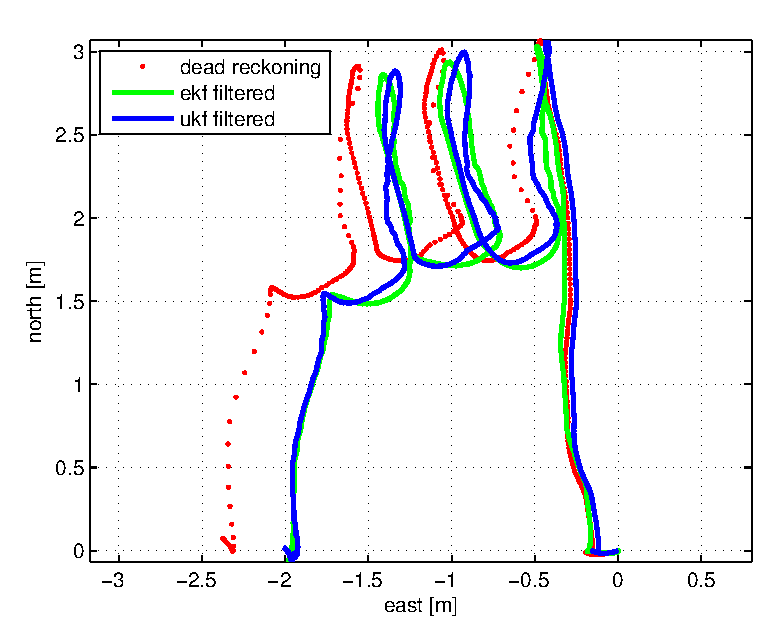
\includegraphics[width=0.42\linewidth]{simulations/fig/UKFpipeTrack.eps}}
    \subfigure[Magnetic disturbances affecting the heading measurement by compass. Vehicle is not moving, FOG is not oscillating at the same time.] {\label{fig:magnetic-disturb}
    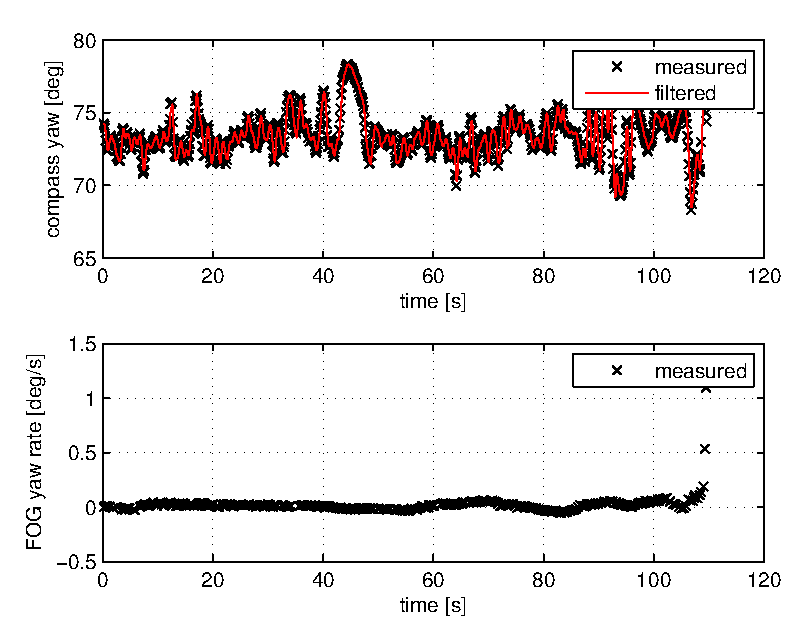
\includegraphics[width=0.42\linewidth]{simulations/fig/magnetic.eps}} 
%\vspace{-33pt}  
\end{figure}